\nonstopmode
\section{Casi d'uso}
\subsection{Scopo}

La presente sezione ha come obiettivo l'identificazione e la descrizione di tutti i casi d'uso individuati dall'analisi del gruppo sul capitolato proposto.

\subsection{Attori}
Come concordato con il proponente, la \emph{webapp}$^{G}$ deve essere utilizzata sia da utenti clienti che da utenti ristoratori, sono stati quindi identificati per il Sistema i seguenti attori:

\begin{itemize}
\item \textbf{Utente non riconosciuto}: è un utente che non ha effettuato l'accesso al Sistema. Può essere sia un utente non registrato sia un utente registrato che non ha ancora effettuato l'accesso.\\ Può ricercare specifici ristoranti e visualizzarli;
\item \textbf{Utente autenticato}: è un utente che ha effettuato l'accesso al Sistema con il proprio \emph{account}$^{G}$ ma non ha ancora selezionato un profilo.\\ Può creare, modificare o eliminare profili cliente o ristoratore;
\item \textbf{Cliente}: è un utente che ha effettuato l'accesso al Sistema ed ha selezionato un profilo cliente.\\ Può effettuare le operazioni di prenotazione ed ordinazione e le loro attività correlate;
\item \textbf{Ristoratore}: è un utente che ha effettuato l'accesso al Sistema ed ha selezionato un profilo ristoratore.\\ Può gestire il proprio ristorante e le prenotazioni ad esso associate.
\end{itemize}
\begin{figure}[h] 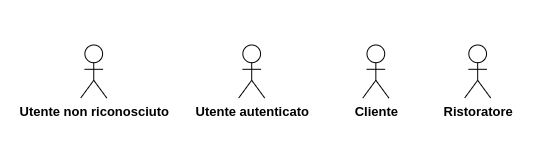
\includegraphics[scale=1]{attori.png} \end{figure}

Non ci sono relazioni di alcun tipo tra i vari attori.

\pagebreak
\subsection{Lista dei casi d'uso}

% registazione - login
<? require_once "src/casi-uso.d/0-utente-non-riconosciuto.tex"; ?>
% profili
<? require_once "src/casi-uso.d/1-utente-autenticato.tex"; ?>
% cliente - navigazione del sito
<? require_once "src/casi-uso.d/2-cliente-prenotazione.tex"; ?>
<? require_once "src/casi-uso.d/3-cliente-ordinazione.tex"; ?>
<? require_once "src/casi-uso.d/4-cliente-altro.tex"; ?>
% ristoratore
<? require_once "src/casi-uso.d/5-ristoratore.tex"; ?>
% chat
<? require_once "src/casi-uso.d/6-cliente-ristoratore-chat.tex"; ?>
